\chapter{Repository instructions and agent configuration}

\section{Engineering principles}

Codex discovers AGENTS.md along its documented directory hierarchy and supports override files. Claude Code loads CLAUDE.md from applicable scopes; direct AGENTS.md discovery is documented for version 2.1.277 and later under specific conditions. If both project files exist, explicit import is a robust compatibility approach, subject to verification on the installed version. Organization-managed settings are distinct from advisory instructions.\src{O2,O4,A2,A10}

\section{Implementation approach}

Keep shared engineering standards in AGENTS.md and Claude-specific guidance in CLAUDE.md using an import. Put service-specific build instructions in the relevant directory only if discovery semantics are confirmed. Review the effective settings at session start. Treat any instruction read from an untrusted branch as data, not authorization. When two instructions conflict, stop and obtain the task owner decision instead of silently selecting the more permissive one.

\section{Verification and limitations}

Create a fixture with conflicting instructions and confirm the approved build command is used. Test permission restrictions separately; a model obeying instructions is not proof of enforcement.

Figure~\ref{fig:d6} illustrates the conceptual flow from Managed / user rules to Effective context. The edges describe the proposed integration or control relationship, not undocumented internal calls.

\begin{figure}[htbp]\centering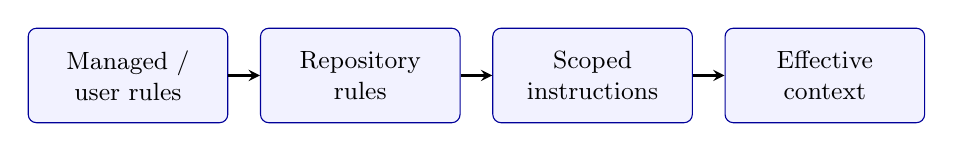
\begin{tikzpicture}[nodebox/.style={draw=blue!60!black,fill=blue!5,rounded corners=3pt,minimum height=12mm,text width=23mm,align=center,font=\small},>=stealth]
\node[nodebox] (n0) at (0.00,0.00) {Managed / user rules};
\node[nodebox] (n1) at (2.95,0.00) {Repository rules};
\node[nodebox] (n2) at (5.90,0.00) {Scoped instructions};
\node[nodebox] (n3) at (8.85,0.00) {Effective context};
\draw[->,thick] (n0.east) -- (n1.west);
\draw[->,thick] (n1.east) -- (n2.west);
\draw[->,thick] (n2.east) -- (n3.west);
\end{tikzpicture}
\caption{Repository instruction discovery (conceptual view).}\label{fig:d6}\end{figure}

\section{Chapter conclusion}

Apply the stated verification criteria before expanding the scope of this workflow. Record deviations, evidence and unresolved risks in the task record.
